% This is "sig-alternate.tex" V1.9 April 2009
% This file should be compiled with V2.4 of "sig-alternate.cls" April 2009
%
% This example file demonstrates the use of the 'sig-alternate.cls'
% V2.4 LaTeX2e document class file. It is for those submitting
% articles to ACM Conference Proceedings WHO DO NOT WISH TO
% STRICTLY ADHERE TO THE SIGS (PUBS-BOARD-ENDORSED) STYLE.
% The 'sig-alternate.cls' file will produce a similar-looking,
% albeit, 'tighter' paper resulting in, invariably, fewer pages.
%
% ----------------------------------------------------------------------------------------------------------------
% This .tex file (and associated .cls V2.4) produces:
%       1) The Permission Statement
%       2) The Conference (location) Info information
%       3) The Copyright Line with ACM data
%       4) NO page numbers
%
% as against the acm_proc_article-sp.cls file which
% DOES NOT produce 1) thru' 3) above.
%
% Using 'sig-alternate.cls' you have control, however, from within
% the source .tex file, over both the CopyrightYear
% (defaulted to 200X) and the ACM Copyright Data
% (defaulted to X-XXXXX-XX-X/XX/XX).
% e.g.
% \CopyrightYear{2007} will cause 2007 to appear in the copyright line.
% \crdata{0-12345-67-8/90/12} will cause 0-12345-67-8/90/12 to appear in the copyright line.
%
% ---------------------------------------------------------------------------------------------------------------
% This .tex source is an example which *does* use
% the .bib file (from which the .bbl file % is produced).
% REMEMBER HOWEVER: After having produced the .bbl file,
% and prior to final submission, you *NEED* to 'insert'
% your .bbl file into your source .tex file so as to provide
% ONE 'self-contained' source file.
%
% ================= IF YOU HAVE QUESTIONS =======================
% Questions regarding the SIGS styles, SIGS policies and
% procedures, Conferences etc. should be sent to
% Adrienne Griscti (griscti@acm.org)
%
% Technical questions _only_ to
% Gerald Murray (murray@hq.acm.org)
% ===============================================================
%
% For tracking purposes - this is V1.9 - April 2009

\documentclass{sig-alternate}
\usepackage{url}
\usepackage{algorithm}
\usepackage[noend]{algorithmic}
\usepackage{subfigure}

%\documentclass{acm_proc_article-sp}
%\def\BibTeX{Bib\TeX}
%\parindent=0pt
%\parskip=\baselineskip

\newcommand{\dae}{{\em Divide-and-Evolve}}
\newcommand{\DAEX}{{\sc DaE$_{\text{X}}$}}
\newcommand{\DAEYAHSP}{{\sc DaE$_{\text{YAHSP}}$}}
\newcommand{\YAHSP}{{\sc YAHSP}}

\begin{document}

%\title{A Multicore Implementation of the Divide-and-Evolve Algorithm}
%\title{Speeding Up the Individual Evaluation of the Divide-and-Evolve Algorithm}
%\title{Multithreading the Divide-and-Evolve Algorithm for a Multicore Machine}
%\title{A Multithreaded Release of the Divide-and-Evolve Planning System for a Multicore Machine}
%\title{A Multicore Implementation of the Individual Evaluation in the Divide-and-Evolve Planner}
\title{Parallel Divide-and-Evolve: Experiments with OpenMP on a Multicore Machine}

\numberofauthors{2} % 4 is a bug!

\author{
\alignauthor
Caner Candan\\
       \affaddr{Thales Research \& Technology}\\
       \affaddr{Palaiseau, France}\\
       \email{caner.candan@thalesgroup.com}
\alignauthor
Johann Dr{\'e}o\\
       \affaddr{Thales Research \& Technology}\\
       \affaddr{Palaiseau, France}\\
       \email{johann.dreo@thalesgroup.com}
\and
\alignauthor
Pierre Sav{\'e}ant\\
       \affaddr{Thales Research \& Technology}\\
       \affaddr{Palaiseau, France}\\
       \email{pierre.saveant@thalesgroup.com}
\alignauthor
Vincent Vidal\\
       \affaddr{ONERA -- DCSD}\\
       \affaddr{Toulouse, France}\\
       \email{vincent.vidal@onera.fr}
}

\maketitle
\begin{abstract}
After having instantiated the evolutionary metaheuristic \DAEX\ with the forward search \YAHSP\ planner, 
we investigate on the global parallelism approach, which exploits the inherent parallelism of the individual evaluation.
This paper describes a parallel shared-memory release of the \DAEYAHSP\ planning system using the OpenMP directive-based API.
The parallelization scheme applies at a high level abstraction and thus can be used by any evolutionary algorithm implemented with the Evolving Objects framework.
The proof of concept is made on a 48-core machine with two planning tasks extracted from the last international planning competition.
Experiments show significant speedups along the number of cores and along the size of the population.


\end{abstract}

\section{Introduction}
Multicore machines are becoming a standard way to speep up the system performance.

% argument : Q=Comment parall�liser un algo de recherche de plans ? 
%            R=concevoir d'abord un algorithme �volutionnaire puis parall�liser sa fonction d'�valuation





Preliminary work


\section{Previous Works in Parallel EA and Parallel Planning}

\paragraph{Parallel EA}

FIXME

\paragraph{Parallel Planning} % (VV)
\label{section:previous-work}

Several  approaches to  parallel planning  have been  proposed in  recent years.
Parallel Retracting A* \cite{PRA-star},  was implemented on a Connection Machine
and  had  to  deal with  very  severe  memory  limitations. In  that  algorithm,
a distributed  hash function is  used to allocate  generated states to  a unique
processing unit  and avoid unnecessary  state duplications. PRA* dealt  with the
memory limitation  through a retraction  mechanism which allowed a  processor to
free its memory by dropping states. In order to confirm the transfer of a state,
synchronous communication channels  had to be used, which  seriously slowed down
the  search  process.  Transposition-table  driven  work scheduling  \cite{TDS},
similarly to PRA* uses a hash function to avoid duplication. It is based on IDA*
and, running  on a  standard architecture, does  not necessitate  any retraction
mechanism  and  can  efficiently  exploit asynchronous  communication  channels.
Parallel  Frontier  A*  with  Delayed  Duplicate  Detection  \cite{PFADDD}  uses
a strategy  based on intervals computed  by sampling to  distribute the workload
among several workstations, targetting  distributed-memory systems as opposed to
previous approaches.  In \cite{HDA-star}, the authors introduce Hash Distributed
A*  (HDA*) which combines  successful ideas  from previous  parallel algorithms.
HDA*  uses a  hash  function which  assigns  each generated  state  to a  unique
processing unit  in order to avoid  the duplication of the  search efforts. This
mechanism  was  introduced  in   PRA*,  which  unfortunately  combined  it  with
synchronous communication channels which caused  a lot of overhead. This problem
was  addressed  in  HDA*  by  the  use  of  non-blocking  communication  (as  in
\cite{TDS}).   In   \cite{burns:ijcai2009,burns:JAIR2010}  the  authors  present
Parallel  Best-NBlock-First (PBNF).   It uses  an abstraction  to  partition the
state space.  PBNF  allows each thread to expand the  most promising nodes while
detecting duplicate states.  Rather than  sleeping if a lock cannot be acquired,
a thread can  perform ``speculative'' expansions by continuing  the expansion of
its current part  of the space.  This technique keeps cores  busy at the expense
of  duplicate work.  \cite{dovetailing}  adapts to  planning a  technique called
dovetailing, in  which several  instances of a  search algorithm  with different
parameter settings  are run in parallel. We  use this approach in  this paper as
a  bottom-line, and show  how our  approach improves  over a  simple dovetailing
strategy.  Finally,  \cite{vidal:socs2010} proposed a multi-core  version of the
YAHSP planner \cite{yahsp:icaps2004} where  many concurrent threads expand nodes
from a common open list, yielding to early exploration of branches of the search
tree that  would have  been delayed  by a classical  search, which  can speed-up
search by several orders of magnitude.

\section{Methods}

\subsection{Algorithms}

\paragraph{Divide and Evolve} % (PS)
% The Planning Problem
The classical planning problem is to find a path in a transition system: a
sequence of actions which maps an initial state $I$ into a state $G$ including a
set of desired goals. Usually a metric is associated with the solution plan such
as length, cost or duration. In domain-independent planning, problems are
described with the Planning Domain Description Language (PDDL)
\cite{pddl:jair2003}; states of the world are defined by a set of atoms
instanciated from a set of predicates and a set of objects. Although there are
several families of problems, we concentrate here on cost planning and temporal
planning. In cost planning a cost is attached to each action and the objective
is to minimize the sum of all costs for a sequential plan whereas in temporal
planning actions have a duration and can be run in parallel. In temporal
planning the objective is to minimize the total makespan of the parallel plan.

% DaE
\DAEX, the concrete implementation of the \dae\ paradigm, is a
domain-independent satisficing planning system based on Evolutionary Computation
\cite{dae:evocop2006}. The basic principle is to carry out a {\em
Divide-and-Conquer} strategy driven by an evolutionary algorithm. The algorithm
is detailed in \cite{dae:icaps2010} and compare with state-of-the-art planners.
In order to solve a planning task ${\cal P}_D(I,G)$, the basic idea of \DAEX\ is
to find a sequence of states $S_1, \ldots, S_n$, and to rely on an embedded
planner $X$ to solve the series of planning tasks ${\cal P}_D(S_{k},S_{k+1})$,
for $k \in [0,n]$ (with $S_0 = I$ and $S_{n+1} = G$).  A \DAEX\ individual is a
sequence of goals which define a sequence of subproblems to be solved. These
subproblems are submitted successively to an embedded planner $X$ and the global
solution is obtained after the compression of these intermediate solutions. The
overall optimization process is controled by an evolutionary algorithm.

The fitness implements a gradient towards feasability for unfeasible individuals
and a gradient towards optimality for feasible individuals. Feasible individuals are always preferred to unfeasible ones.
Population initialization as well as variation operators are driven by the critical path
$h^1$ heuristic \cite{h1:aips2000} in order to discard inconsistent state
orderings, and atom mutual exclusivity inference in order to discard
inconsistent states. Beside a standard one-point crossover for variable length
representations, four mutations have been defined: addition (resp. removal) of a
goal in a sequence, addition (resp. removal) of an atom in a goal. The
selection is a comparison-based deterministic tournament of size 5.

% Parameter tuning
For the sequential release, Darwinian-related parameters of \DAEX\ have been
fixed after some early experiments \cite{dae:evocop2006} whereas parameters
related to the variation operators have been tuned using the Racing method
\cite{dae:gecco2010}.

All experiments were done with \DAEYAHSP: the instantiation of \DAEX\ with the
YAHSP heuristic forward search solver \cite{yahsp:icaps2004}. % + YAHSP memoing
shared by all searches.  We added two novelties to the version described in
\cite{dae:icaps2010}.  One important parameter is the maximum number of expanded
nodes allowed to the \YAHSP\ sub-solver which defines empirically what is
considered as an easy problem for \YAHSP. As the matter of fact, the minimum
number of required nodes varies from few nodes to thousands depending of the
planning task.  In the current release this number is estimated during the
population initialization stage. An incremental loop is performed until the
ratio of feasible individals is over a given theshold or a maximum boundary has
been reached. By default this number is doubled at each iteration until at least
one feasible individual is produced or 100000 has been reached.

Furthermore we add the capability to perform restarts within a time contract in
order to increase solution quality.

\paragraph{Yet Another Heuristic Search Planner} % (VV)

The YAHSP planning system 
\cite{yahsp:icaps2004}  extends  a  technique   introduced  in  the  FF  planner
\cite{ff:jair01}  for calculating  the  heuristic, based  on  the extraction  of
a solution  from a planning graph  computed for the relaxed  problem obtained by
ignoring deletes of actions.  It can  be performed in polynomial time and space,
and  the length in  number of  actions of  the relaxed  plan extracted  from the
planning  graph represents  the heuristic  value of  the evaluated  state.  This
heuristic  is used  in  a  forward-chaining search  algorithm  to evaluate  each
encountered state.

A novel  way has been  introduced in YAHSP  for extracting information  from the
computation of  the heuristic,  by considering the  high quality of  the relaxed
plans  extracted by  the heuristic  function in  numerous domains.   Indeed, the
beginning of these plans can often  be extended to solution plans of the initial
problem, and there  are often a lot  of other actions from these  plans that can
effectively be  used in a solution  plan. YAHSP uses an  algorithm for combining
some actions from each  relaxed plan, in order to find the  beginning of a valid
plan that can lead to a reachable  state. Thanks to the quality of the extracted
relaxed  plans,  these states  frequently  guide  search  closer to  a  solution
state. The lookahead states thus calculated  are then added to the list of nodes
that can be chosen to be expanded  by increasing order of the numerical value of
the  heuristic.

This lookahead  strategy can be used  in different search  algorithms. In YAHSP,
a classical  best-first search algorithm  has been modified  in such a  way that
completeness is preserved.   It simply consists in augmenting  the list of nodes
to be  expanded (the open  list) with some  new nodes computed by  the lookahead
algorithm.  The branching factor is slightly increased, but the performances are
generally better and completeness is not affected.

A first motivation in  the use of YAHSP in \DAEX\ is  that experiments about the
use of  this lookahead strategy in  a complete best-first  search algorithm have
demonstrated that in numerous planning benchmark domains, the improvement of the
performance in  terms of running time and  size of problems that  can be handled
are been  drastically improved (cf. \cite{yahsp:icaps2004}).   The YAHSP planner
has been  awarded a second place  in the $4^{th}$  International Planning Competition
\cite{ipc4:jair05} and some  recent results \cite{rintanen:acai2010} demonstrate
that  it is still  extremely competitive  with more  recent planners.   A second
motivation in the use  of YAHSP in \DAEX\ is its ability  to answer very fast to
the considerable number of planning requests emanating from \DAEX, as opposed to
modern  techniques such  as  the  landmark heuristics  implemented  in the  LAMA
planner   \cite{lama:jair2010}  (winner  of   the  $6^{th}$   International  Planning
Competition) which require a costly analysis for each new initial state.

\paragraph{Parts that can theoretically be parallelized} %  (JD, VV, PS)

As  shown in  Section \ref{section:previous-work},  heuristic  search algorithms
used in automated  AI planners can be parallelized in  many ways, although there
is no obvious and  natural way to do so.  However, our goal  in this work is not
to  parallelize the  underlying planner,  but the  evolutionary  algorithm which
controls the  planner, which can  be made in  a very efficient way.   Indeed, in
typical  population-based  algorithms   such  as  evolutionary  algorithms,  the
evaluation of individuals can be made independently of each other, a fortiori in
a parallel way.  Applying variation operators can also be performed in parallel;
and  depending  on  the  application,  parallelism  on  variation  operators  or
individual  evaluation will  have a  different impact  on the  running  time and
utilization  of the  computational  resources.  In \DAEX,  the  running time  of
applying the variation operators is negligible w.r.t.  the running time required
by the individual evaluations by an embedded planner, which is the reason why we
only parallelized the latter.

% Correctness of the \DAEYAHSP\ parallel release
% Burns et al.:
%Soundness: Soundness holds trivially because no solution is returned that does not pass the goal test.
%Deadlock: There is only one lock in PBNF and the thread that currently holds it never attempts to acquire it a secondtime, so deadlock cannot arise.
%Livelock:
%Completeness This follows easily from liveness:

% Wikipedia: 
%A deadlock is a situation where in two or more competing actions are each waiting for the other to finish, and thus neither ever does.
%A livelock is similar to a deadlock, except that the states of the processes involved in the livelock constantly change with regard to one another, none progressing. Livelock is a special case of resource starvation; the general definition only states that a specific process is not progressing.
%A real-world example of livelock occurs when two people meet in a narrow corridor, and each tries to be polite by moving aside to let the other pass, but they end up swaying from side to side without making any progress because they both repeatedly move the same way at the same time.
%Livelock is a risk with some algorithms that detect and recover from deadlock. If more than one process takes action, the deadlock detection algorithm can be repeatedly triggered. This can be avoided by ensuring that only one process (chosen randomly or by priority) takes action


\subsection{Implementation}

\paragraph{Locks, thread-safe \& reentrant subroutines} % (VV)

Even  if  being  very  natural   in  the  context  of  evolutionary  algorithms,
parallelizing individual evaluations in \DAEX\  requires to be carefully made in
order to avoid some typical problems that can happen with shared-memory parallel
implementations.  Indeed,  even if  the evaluation of  the individuals  are made
independently of each  other, some concurrent access to  shared memory are still
required  (for  example, a  basic  one  is  incrementing some  global  counter),
especially in YAHSP (detailed below). Furthermore, the implementations of \DAEX\
and  YAHSP where  not  designed with  parallelism  in mind,  which implied  some
modifications to render them thread-safe.

One first problem that can  happen in a shared-memory parallel implementation is
\emph{deadlocks}, which are situations where at least two concurrent threads are
each waiting  for the  other to finish,  and thus  neither ever does.   This can
happen for example when a thread $t_1$ acquires a lock on a shared variable $x$,
and then tries  to acquire a lock  on another shared variable $y$;  while in the
same time a thread $t_2$ acquired a lock on $y$ and then tries to acquire a lock
on $x$.  Each thread  waiting for the other one to release  the lock on the next
variable locked by the other  thread, nothing happens.  A variation of deadlocks
is \emph{livelocks},  where the  threads are still  able to continue  doing some
work but cannot go through some portion of the code due to a similar phenomenon.

Another problem  that can arise is the  concurrent use of a  given subroutine by
several threads, when such a subroutine or some subroutine called by it modifies
some  global data.   This is  a  typical problem  of reentrancy,  which must  be
carefully analyzed in order to render thread-safe a parallel implementation. Two
cases can then occur: either the  global data must shared by some threads, which
requires to protect its  access, or it can be made private  to each thread, thus
necessitating to change the scope of this data.

\paragraph{EO \& OpenMP} % (CC, JD)

%\subparagraph{Evolving Object, an evolutionary computation framework}\\
%\DAEYAHSP\ has been implemented within the Evolving Objects framework (\url{http://eodev.sourceforge.net/}), an Open Source, STL-based, C++ Evolutionary Computation library. 

Standing for Evolving Object\footnote{Evolving Object:
\url{http://eodev.sf.net}}, EO is largely used and known framework in
evolutionary computation based on template approach in C++. It helps at
designing evolutionary algorithms for hard optimization problems, from
continuous to combinatorial ones.

An extension of EO for parallelization of algorithms, ParadisEO, has been
proposed by Cahon et al. \cite{paradiseo:JHeuristics2004}. It uses the Message
Passing Interface API and proposes several parallelization scheme, available by
calling wrappers around common functions of EO. We have choose not to use this
framework because we were targeting multicore architecture, where message
passing is useless and may introduce an overhead higher than other approaches. 

%\subparagraph{OpenMP and parallelization paradigms}\\

For multicore architecture, shared memory parallelization approach is a better
candidate. In this work, we have used OpenMP\footnote{OpenMP: \url{http://www.openmp.org}}.
%The choice between the both shared memory and distributed paradigms has been done with OpenMP according to our resources used for experiences which is only one machine. This is going to be explained in further details later.

% parler de la genericite de la technique de parallelisation, n'importe qui peut utiliser EO pour avoir du code parallel independament de DaE/Yahsp.

In order to parallelize a large scope of the framework EO, an analyze was done
to identify the most used resources by almost all structures. Most of the EO
classes use the ``Functor''\footnote{Also called function object} pattern. The
advantages of this design is to get the genericity and the benefits given by
classes while keeping the simplicity of a single call to a function. EO Functors
generaly take a population as argument.

Considering that the evaluation of the population is the most costly part of the
algorithm, this step is our first target to parallelize. Moreover, in most cases
the evaluation done on individuals can be made in parallel without data
dependencies.  There are several classes in EO implementing evaluation operators
but all of them call a common function to apply the evaluation on a population,
this is the function ``apply''.

\paragraph{EO::apply} % (CC)
%\footnote{Look at the header file apply.h available in the sources of EO}
The function called ``apply'' takes as parameters a population and a function to apply to each individual.

%% TODO: refaire algo proprement avec algorithm2e

\vspace{-0.2cm}
\begin{algorithm}[h!]
\caption{apply(proc, pop)}
\vspace{0.2cm}
\begin{verbatim}
template < typename EOT >
void apply< EOT >( eoUF< EOT, void >& proc,
                   std::vector< EOT >& pop )
{
  for ( size_t i = 0; i < pop.size(); ++i )
    proc( pop[i] );
}
\end{verbatim}
\end{algorithm}
\vspace{-0.2cm}

%% Here is the pseudo code of this function:
% \begin{algorithmic}
  % \WHILE {$i\geq population size$}
  % \STATE $$
  % \ENDWHILE
% \end{algorithmic}

The parallelization of this region of code is done thanks to the pragma ``omp for''. This can be translated in the PRAM model by the use of CREW\footnote{CREW: Concurantial Read Exclusive Write} model.

%%According to the PRAM\footnote{wikipedia PRAM} models we are using a CREW\footnote{Concurantial Read Exclusive Write} model.

%% TODO: refaire algo proprement avec algorithm2e

\vspace{-0.2cm}
\begin{algorithm}[h!]
\caption{apply(proc, pop) parallelized using OpenMP directives}
\vspace{0.2cm}
\begin{verbatim}
template < typename EOT >
void apply< EOT >( eoUF< EOT, void >& proc,
                   std::vector< EOT >& pop )
{
#pragma omp for
  for ( size_t i = 0; i < pop.size(); ++i )
    proc( pop[i] );
}
\end{verbatim}
\end{algorithm}
\vspace{-0.2cm}

In order to permits OpenMP to build a multithreaded algorithm without side
effects, the evaluation functor (the ``proc'' in the apply function) must fulfil certain requirement. 
In EO, the evaluation functors are supposed to be instanciated only once. In a
sequential mode, the same instance is used to evaluate every individuals in a
population. In a parallelized mode, one must ensure that the evaluation functor
have thread-local data structures.

When parallelizing the evaluation loop in an evolutionary algorithm, there
exists a synchronization step at each iteration, this ensure that no race-condition
may occurs. Indeed, individuals being evaluated are all independent, which is
the case in the majority of evolutionary algorithm, and also in \DAEX.

\paragraph{YAHSP \& OpenMP} % (VV)

The design  of YAHSP has  been made in  C with efficiency  in mind, and  kept as
light as  possible. This is typically  the kind of  implementation, making heavy
use of global  variables, not designed for a concurrent  use by several parallel
threads, and where thread-safety is clearly not ensured.  However, OpenMP offers
a facility  to deal with global variables,  in order to change  their scope: the
``omp threadprivate'' pragma.  It takes  as parameter a list of global variables
whose  scope must  be changed  from shared  by all  threads to  private  to each
thread.   And  finally, specifying  which  global  variable  should be  rendered
private to each thread  was the only thing we had to  do to ensure thread-safety
in YAHSP.   For example, the  global arrays used  to compute the  heuristic, the
relaxed plans and the lookahead plans  are made private to each thread, ensuring
that concurrent  excutions of YAHSP do not  use the same portions  of the global
memory.

\paragraph{\DAEX-Specific Parallelization Issues} % (JD)

\DAEX evaluation step calls the YAHSP solver several times on the same
decomposition and thus uses several variables to keep the state of the
evaluation over the searches between intermediate goals (namely $k$, $B$ and
$U$).  As the evaluation functor is a single instance, it must be guaranted
reentrant and not use static variables nor attributes. A way to achieve the
re-entrancy is to define those variables as attributes of the decomposition
itself, and not as attributes of the evaluation functor.



\section{Experimental Study}

\subsection{Setup}

\paragraph{Hardware} % (PS)
The algorithm is programmed in C++ using the GNU OpenMP threading library (GOMP) and run on a 48-core DELL PowerEdge R815 Rack Server set up with four 12-core AMD Opteron(tm) 6174, 2.2GHz (12x512 KB cache) processors with 192GB of RAM.

\paragraph{Benchmarks} % (PS)
We have tested the above implementation on two benchmarks from the satisficing track of the $6^{th}$ International Planning Competition\footnote{\url{http://ipc.icaps-conference.org}}: Elevators-12 for cost planning and Openstacks-17 for temporal planning.

The elevators domain is stated as follows: there is a building with N+1 floors, numbered from 0 to N. The building can be separated in blocks of size M+1, where M divides N. Adjacent blocks have a common floor. The building has K fast (accelarating) elevators that stop only in floors that are multiple of M/2 (so M has to be an even number). Each fast elevator has a capacity of X persons. Furthermore, within each block, there are L slow elevators, that stop at every floor of the block. Each slow elevator has a capacity of Y persons (usually Y<X).
There are costs associated with each elavator starting/stoping and moving. There are several passengers, for which their current location and their destination are given.
The objective function is to minimize the total cost of moving the passengers to their destinations. The total cost is increased each time an elevator starts/stops or moves.

The openstacks domain is based on the "minimum maximum simultaneous open stacks" combinatorial optimization problem, which can be stated as follows: a manufacturer has a number of orders, each for a combination of different products, and can only make one product at a time. The problem is to order the making of the different products so that the maximum number of stacks that are in use simultaneously, or equivalently the number of orders that are in simultaneous production, is minimized. The problem is NP-hard and known to be equivalent to several other problems. In the temporal case a maximum number of stacks is given and the goal is to find the plan with the least makespan, without violating the maximum number of stacks constraints.


\paragraph{Algorithm Parameters} % (PS)

All the experiments were done with the parameter set described in \cite{dae:icaps2010} except for the population size which varies according to the experiment.
The fixed evolution engine is a (pop size+ $7 \times$ pop size)-ES: $n$ individuals generate $7 \times n$ offsprings without selection.
For all runs, the following steady-state stopping condition has been applied: after at least 10 generations, evolution is stopped if no improvement of the best fitness in the
population is made during 50 generations, with a maximum of 1000 generations.

\subsection{Results}

% FIXME: in restart mode an instance launched with more than 1 thread stops before the 30 minutes defined with --max-seconds, Pierre things that the reason is because the time is defined in user-time and not in wall-clock.

% FIXME: .out empty, why ?!?

\paragraph{Measures}

% wall-clock: pourquoi wall-clock est pas user-time ...
% lister les mesures

Here is the three equations of measure used: the speedup, the efficiency and the advanced speedup introduced by the Amdhal's law.

$$Speedup\ measure = r \sum^{P,d}_{k=0,l=0} S_{p_{kl}}$$

according to the speedup equation: $S_p = \frac{T^*_1}{T_p}$

we get the following equation:

$$Speedup\ measure = r \sum^{P,d}_{k=0,l=0} \frac{T^*_{1_{kl}}}{T_{p_{kl}}}$$

The efficiency measure equation is the following.

$$Efficiency\ measure = r \sum^{P,d}_{k=0,l=0} E_{p_{kl}}$$

And finally the advanced speedup provided by Amdhal's law:

$$A_p = \frac{1}{(1-s) + \frac{s}{p}}$$

$s$ being the parallelizable part of the program and $p$ the number of cores used.

This equation allows to extract the sequential part of the program not parallelized and what ever number of cores we use, this sequential part will still be there.

The limit of $A_p$ as $p$ approaches infinity is equal to the sequential part of the program.

$$\lim_{p \to \infty} A_p = \frac{1}{(1-s)}$$

%% Results
\paragraph{Speed-up against nb of cores} % (CC, JD)

\begin{figure}[htpb]
  \begin{center}
    \subfigure[elevators 12]{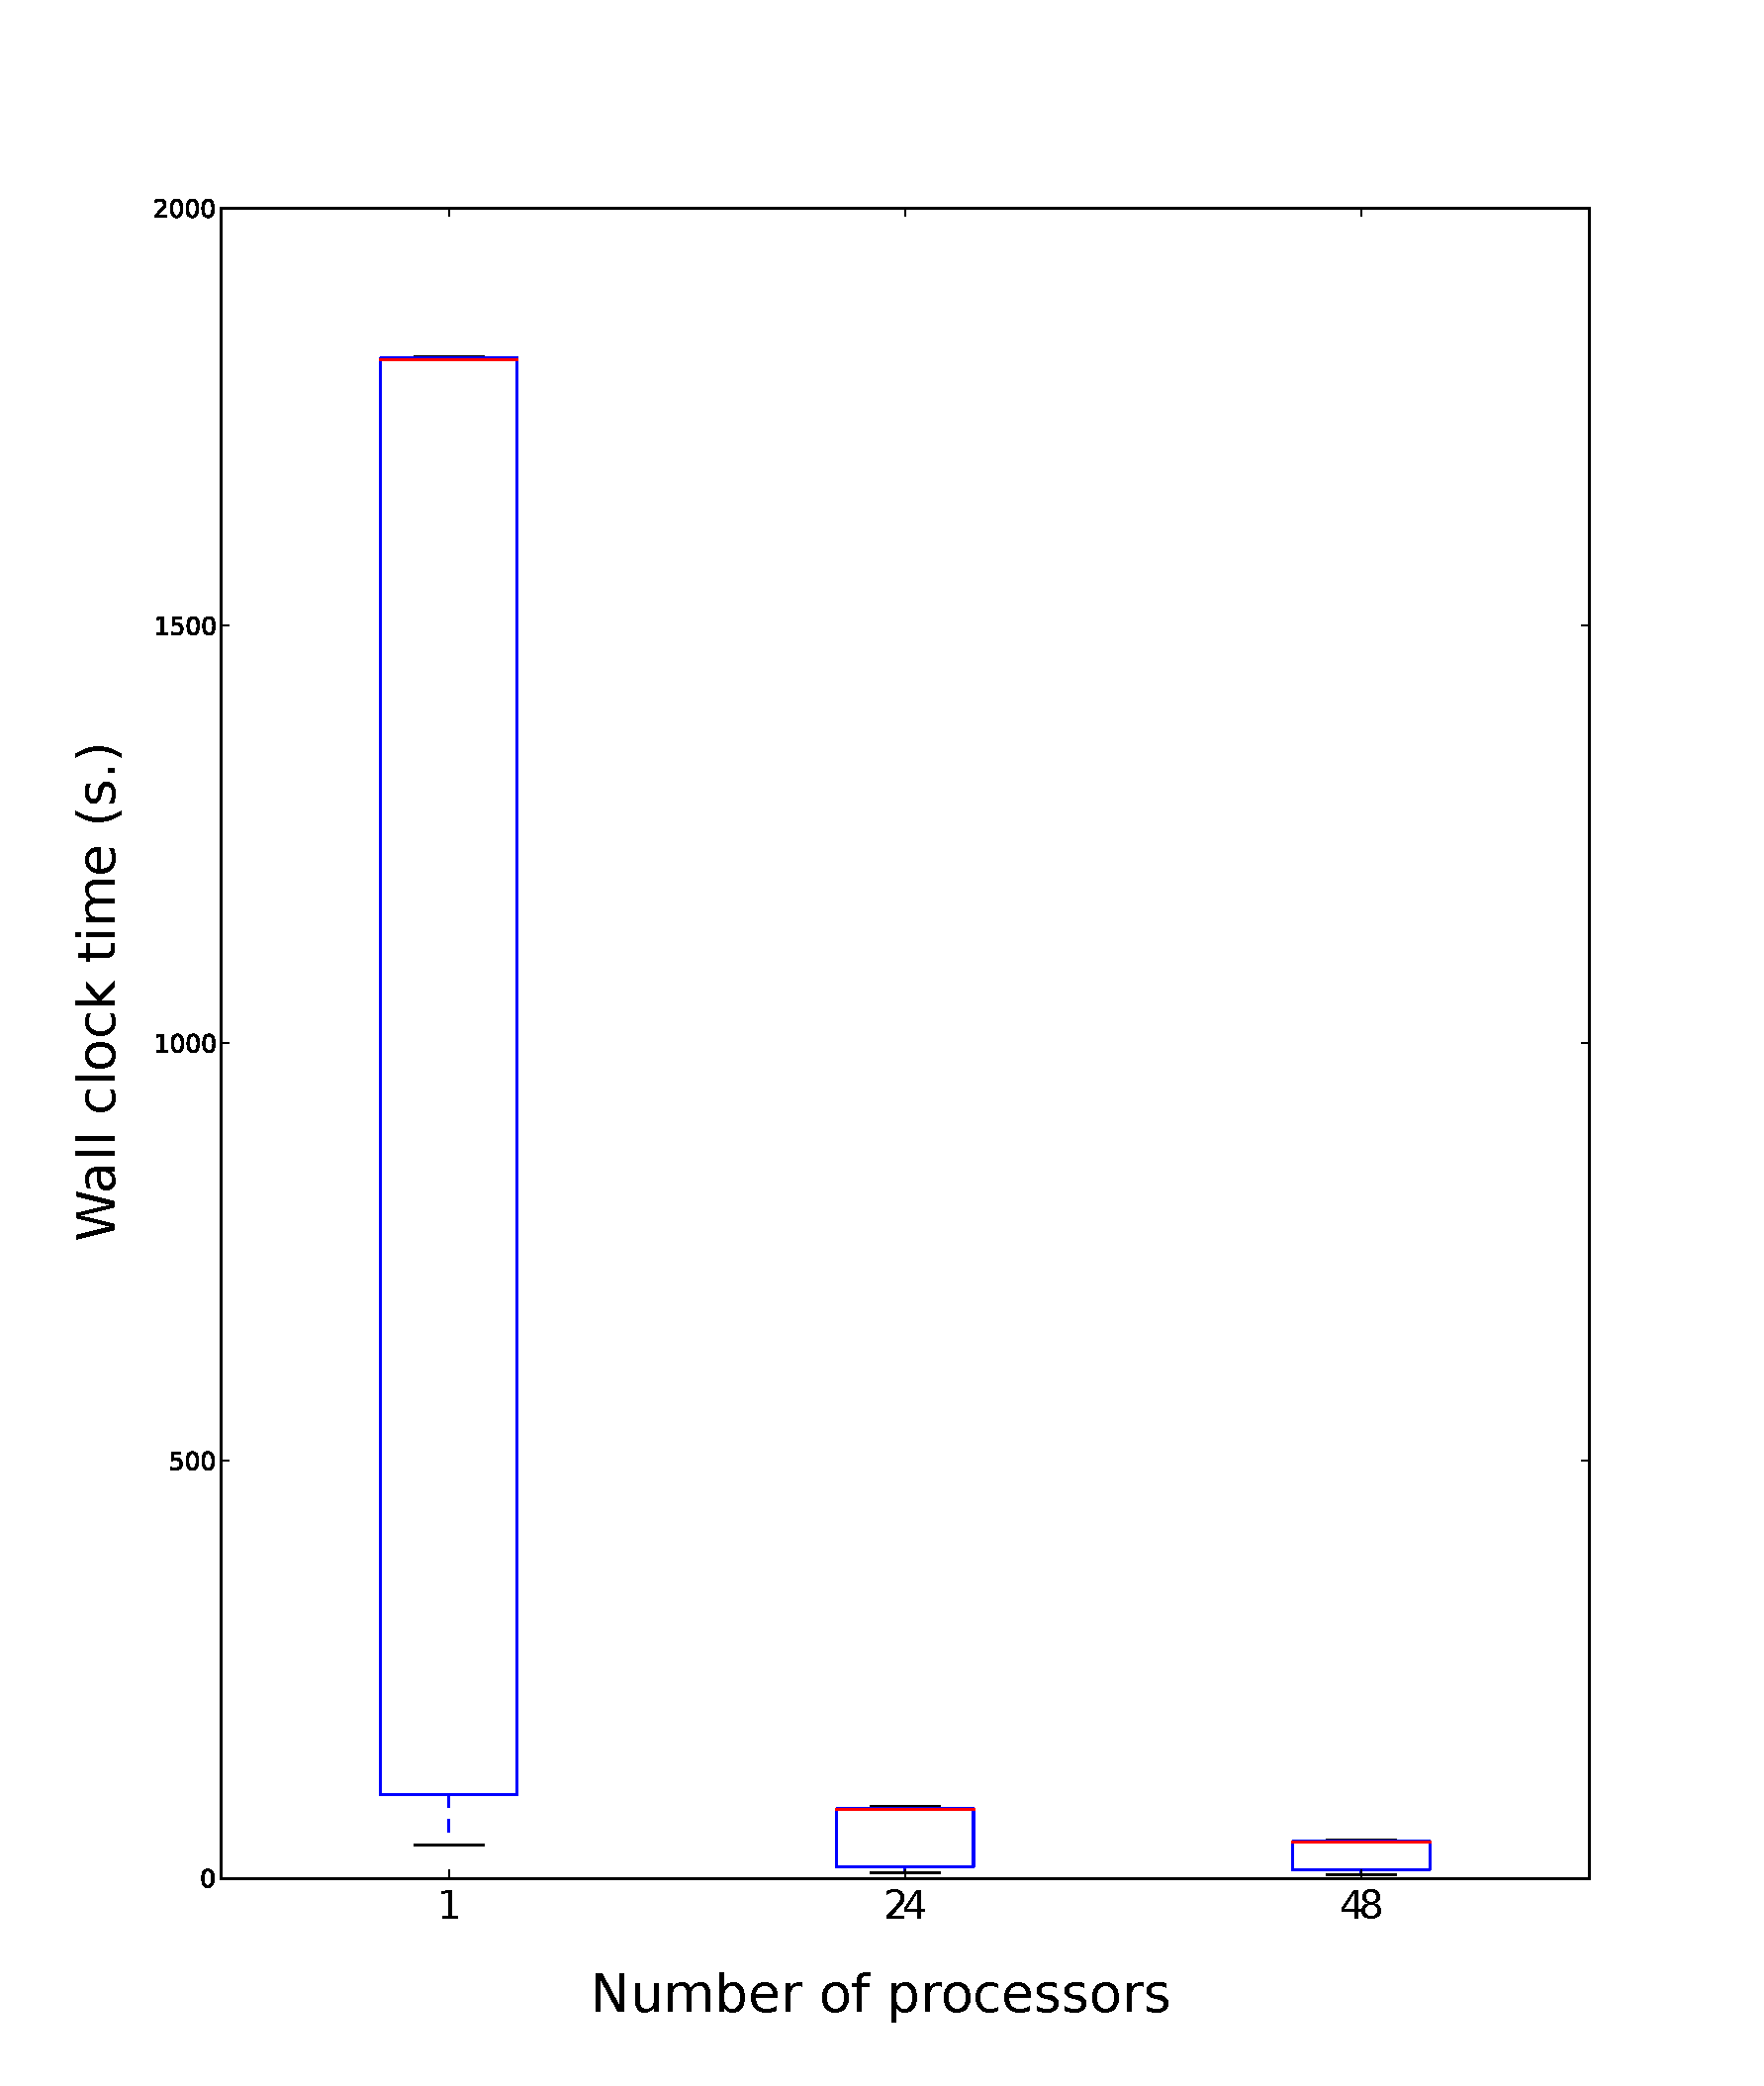
\includegraphics[width=0.2\textwidth]{images/elevators_proc_time.pdf}}
    \hfill
    \subfigure[openstacks 17]{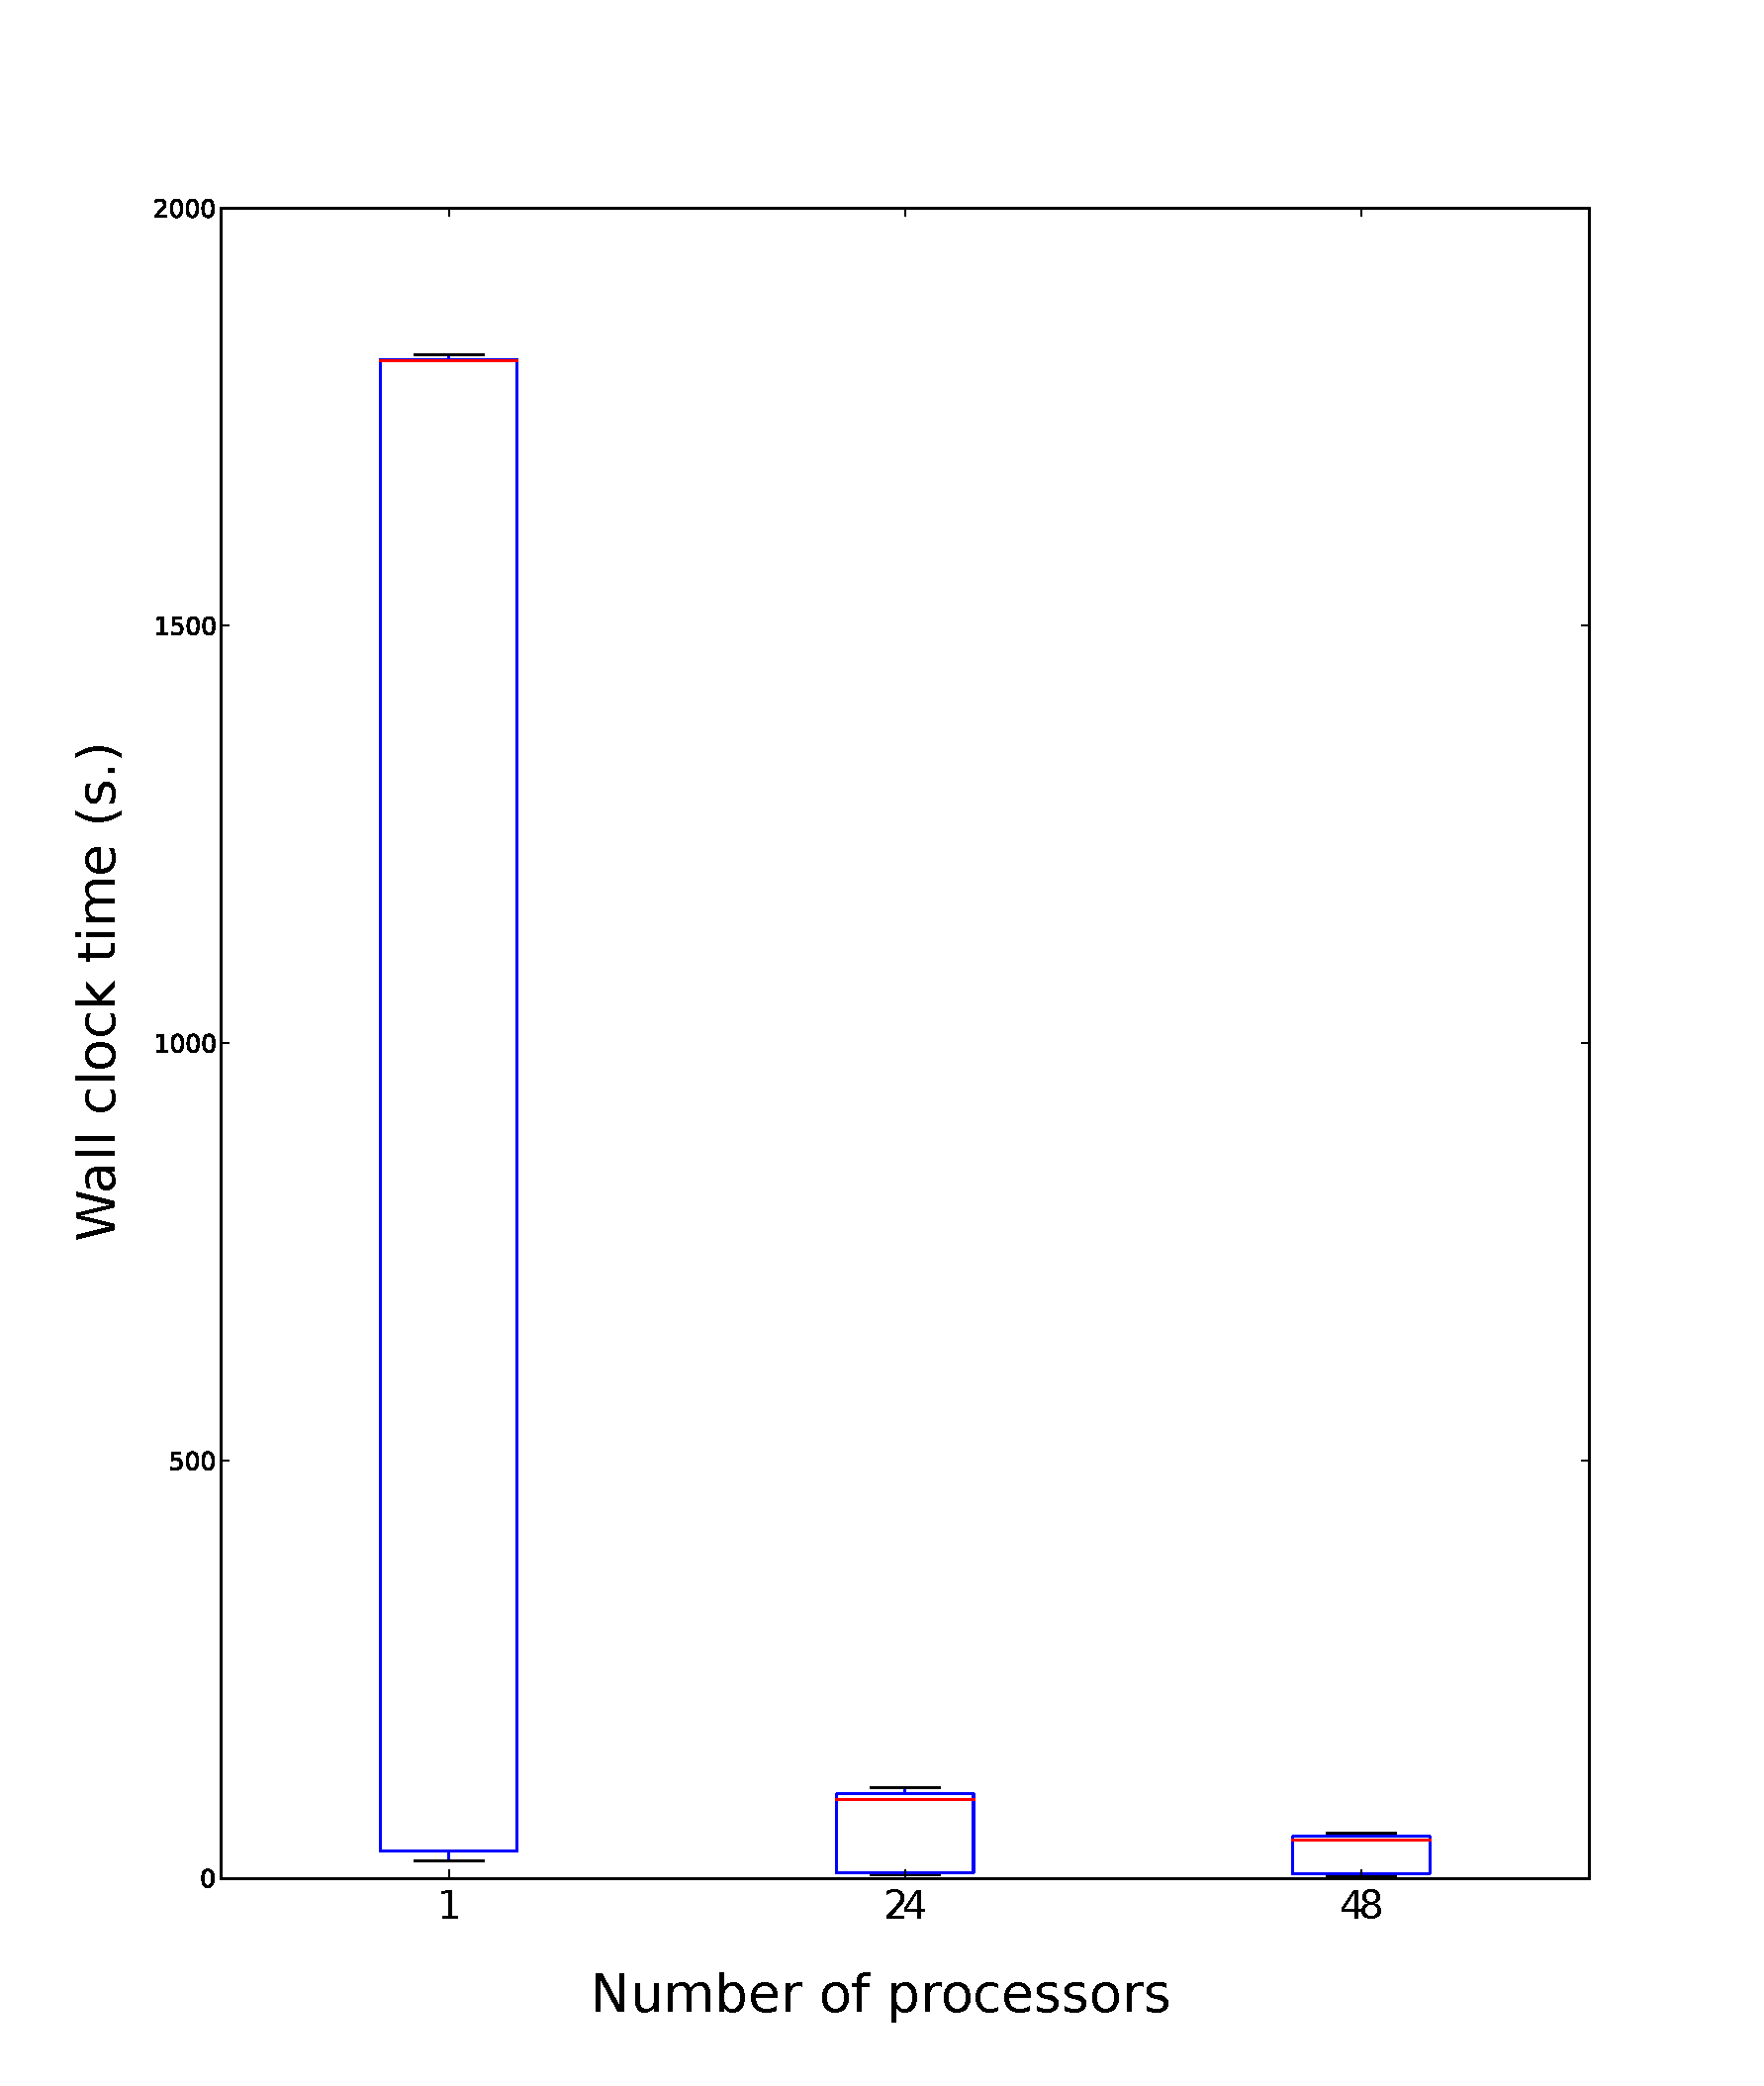
\includegraphics[width=0.2\textwidth]{images/openstacks_proc_time_dynamic.pdf}}
  \end{center}
  \caption{Absolute wallclock time distributions of 11 runs of \DAEYAHSP\ according to the number of processors.}
  \label{fig:proc_elevators_vs_openstacks}
\end{figure}

Figure \ref{fig:proc_elevators_vs_openstacks} shows that on both problems, the
computation time decrease with the number of processors used. Comparing to the
sequential version (running on a single processor), the parallel one permit a
decrease that is similar on both problems. The dispersions of the distribution 
is due to the steady-state stopping criterion that may be reached after different
times.

\paragraph{Comparaison of Static and Dynamic Scheduling} % (CC, JD)

OpenMP lets the choice between the both static and dynamic task scheduling. The default one is the static scheduling.

%static scheduling

To iterate through a set of tasks we divide the number of tasks by the number of processus available. This means that each processus has some defined tasks to accomplish.

%dynamic scheduling

Regarding dynamic scheduling, during the runtime if one processus has finished these tasks it is going to work on another task available. It is similar to a tasks' queue.

% As the goal is to optimize the time cost used by a problem solved in a variable time, we have to verify whether the dynamic scheduling brings a better efficiency.

% some hypotheses

Two hypotheses have driven us to test the dynamic scheduling. The first one consists to say that as long as we are using a problem solved in a variable time, the dynamic scheduling should be faster than the static scheduling does. The second one assumes that we use a population size higher than the number of cores available, the dynamic mode should bring a better efficiency.

% less time consuming

To determine the quality of the dynamicity in front of statical schedule, we are using the following formula:

$$D_p = \frac{S^s_p}{S^d_p}$$

$S^s_p$ is the speedup for the static scheduling.\\
$S^d_p$ is the speedup for the dynamic one.\\


\begin{figure}[htpb]
  \begin{center}
    \subfigure[static]{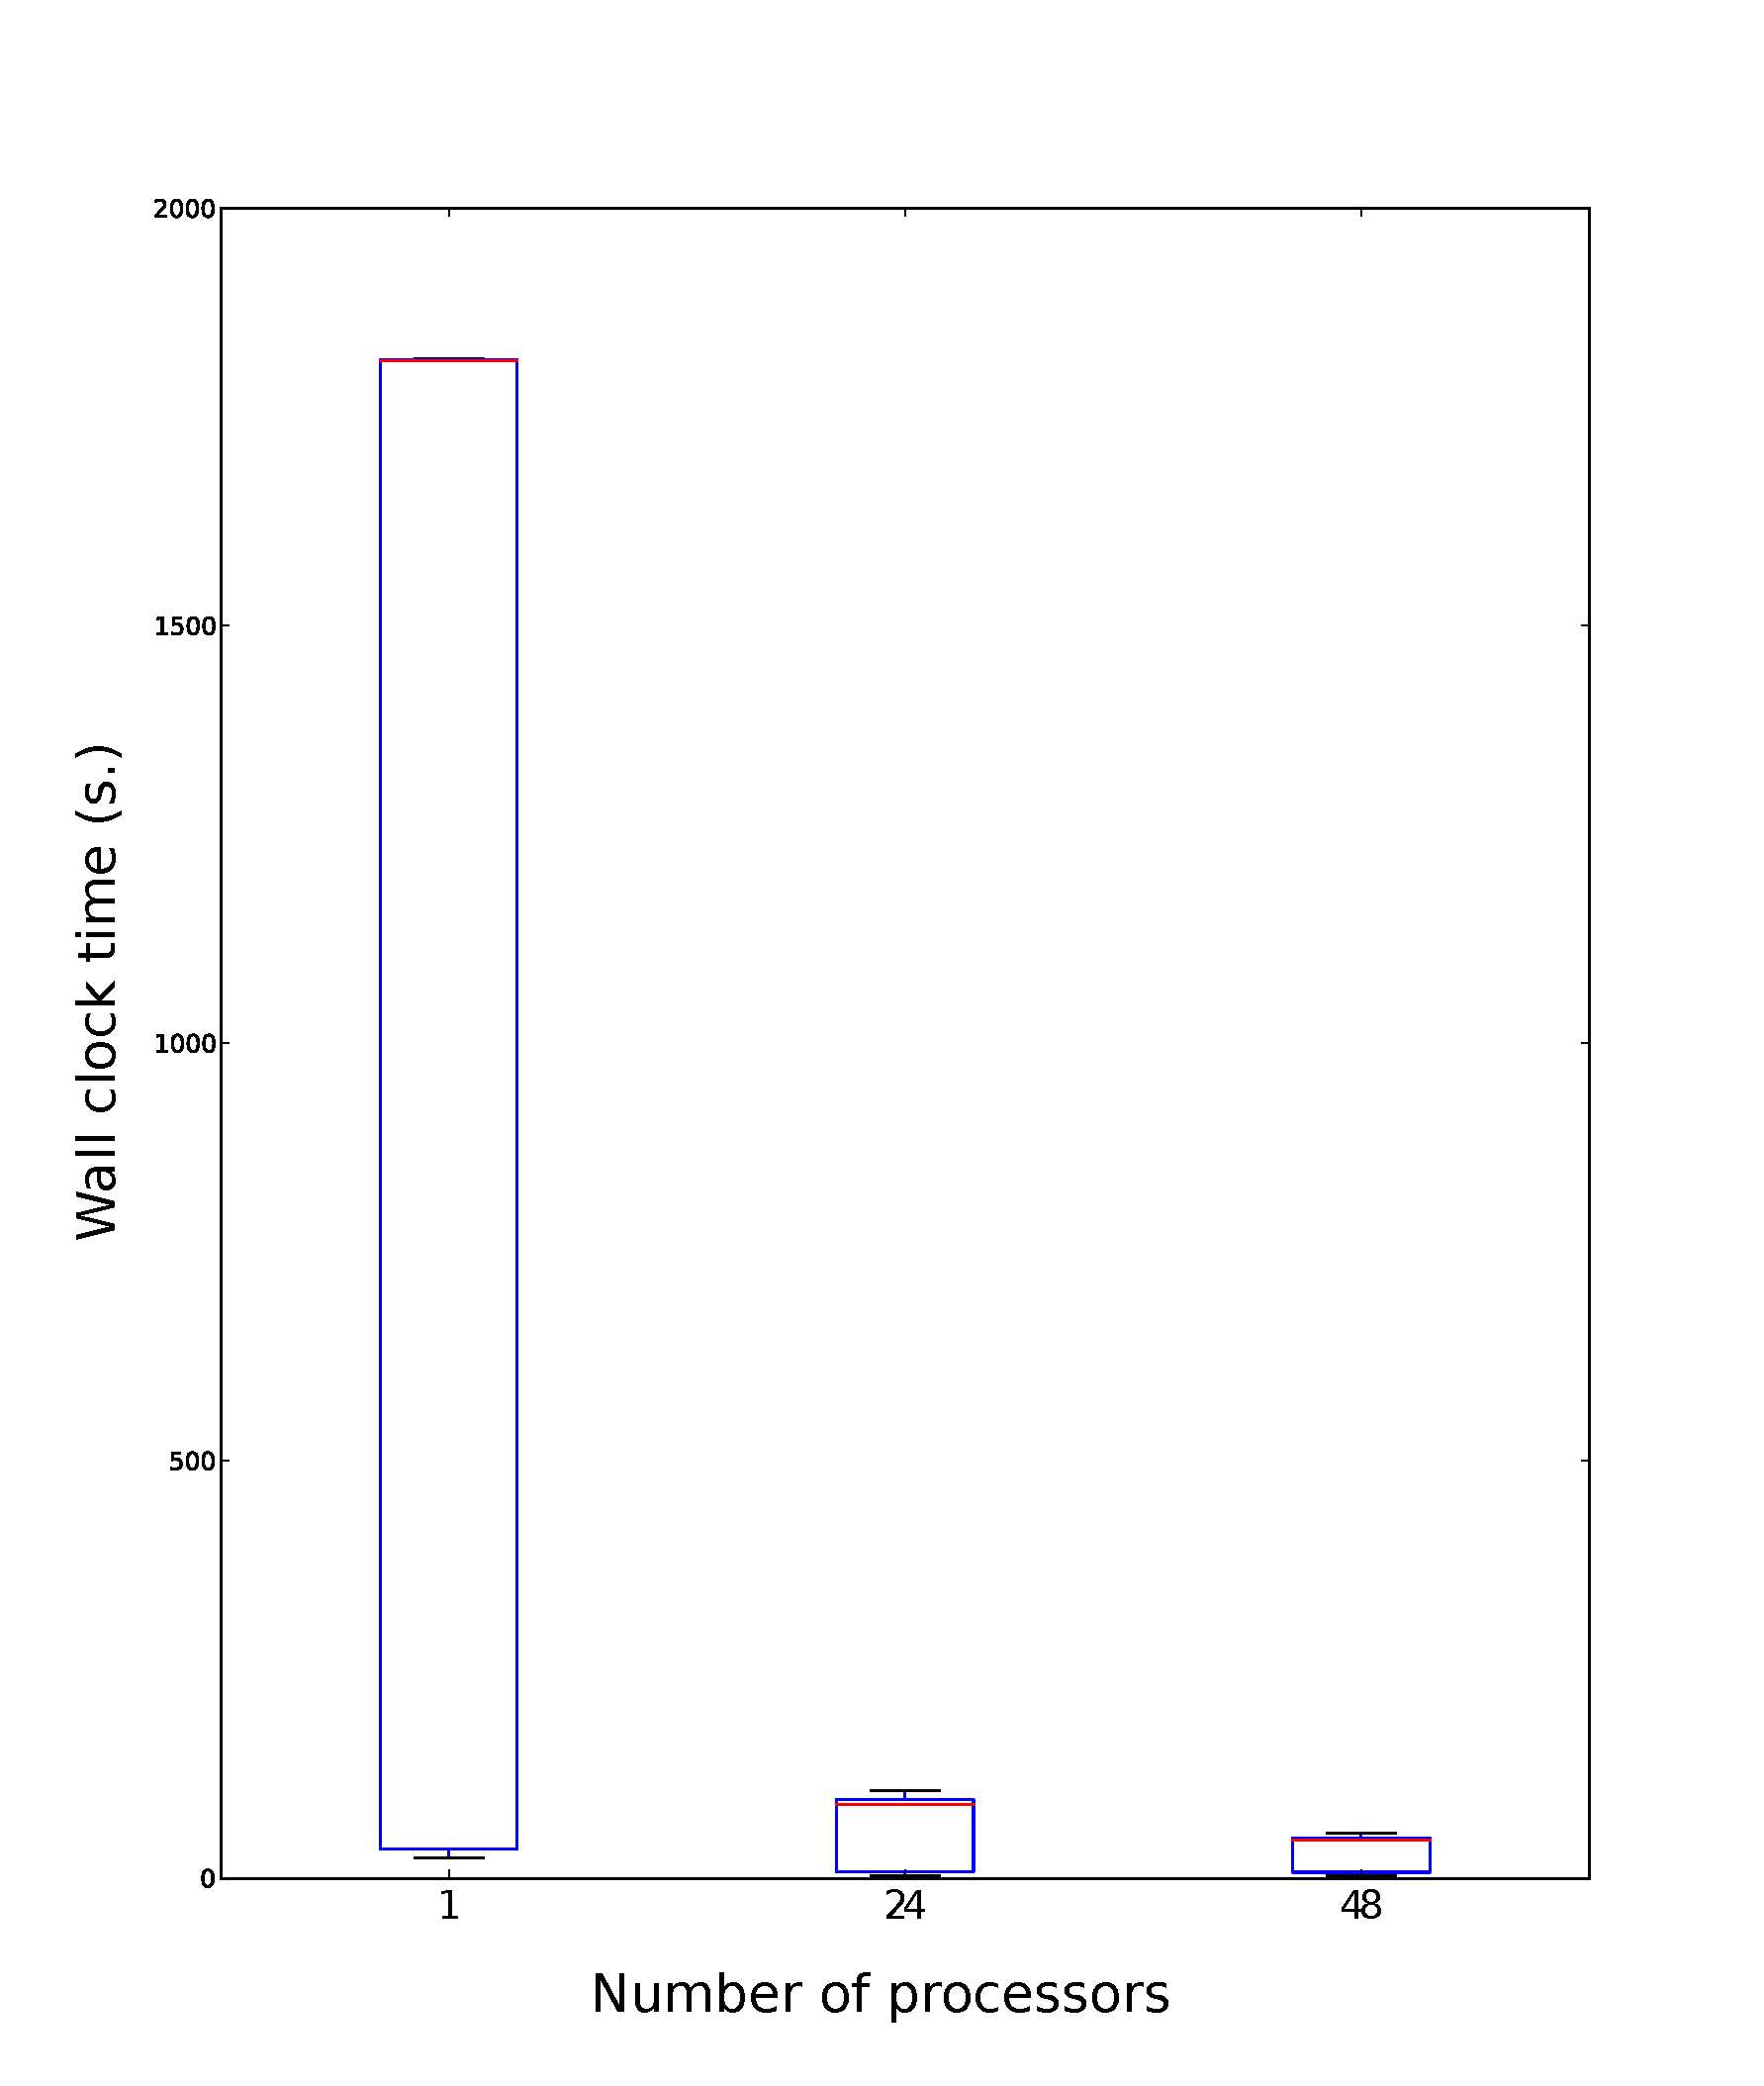
\includegraphics[width=0.2\textwidth]{images/openstacks_proc_time_static.pdf}}
    \hfill
    \subfigure[dynamic]{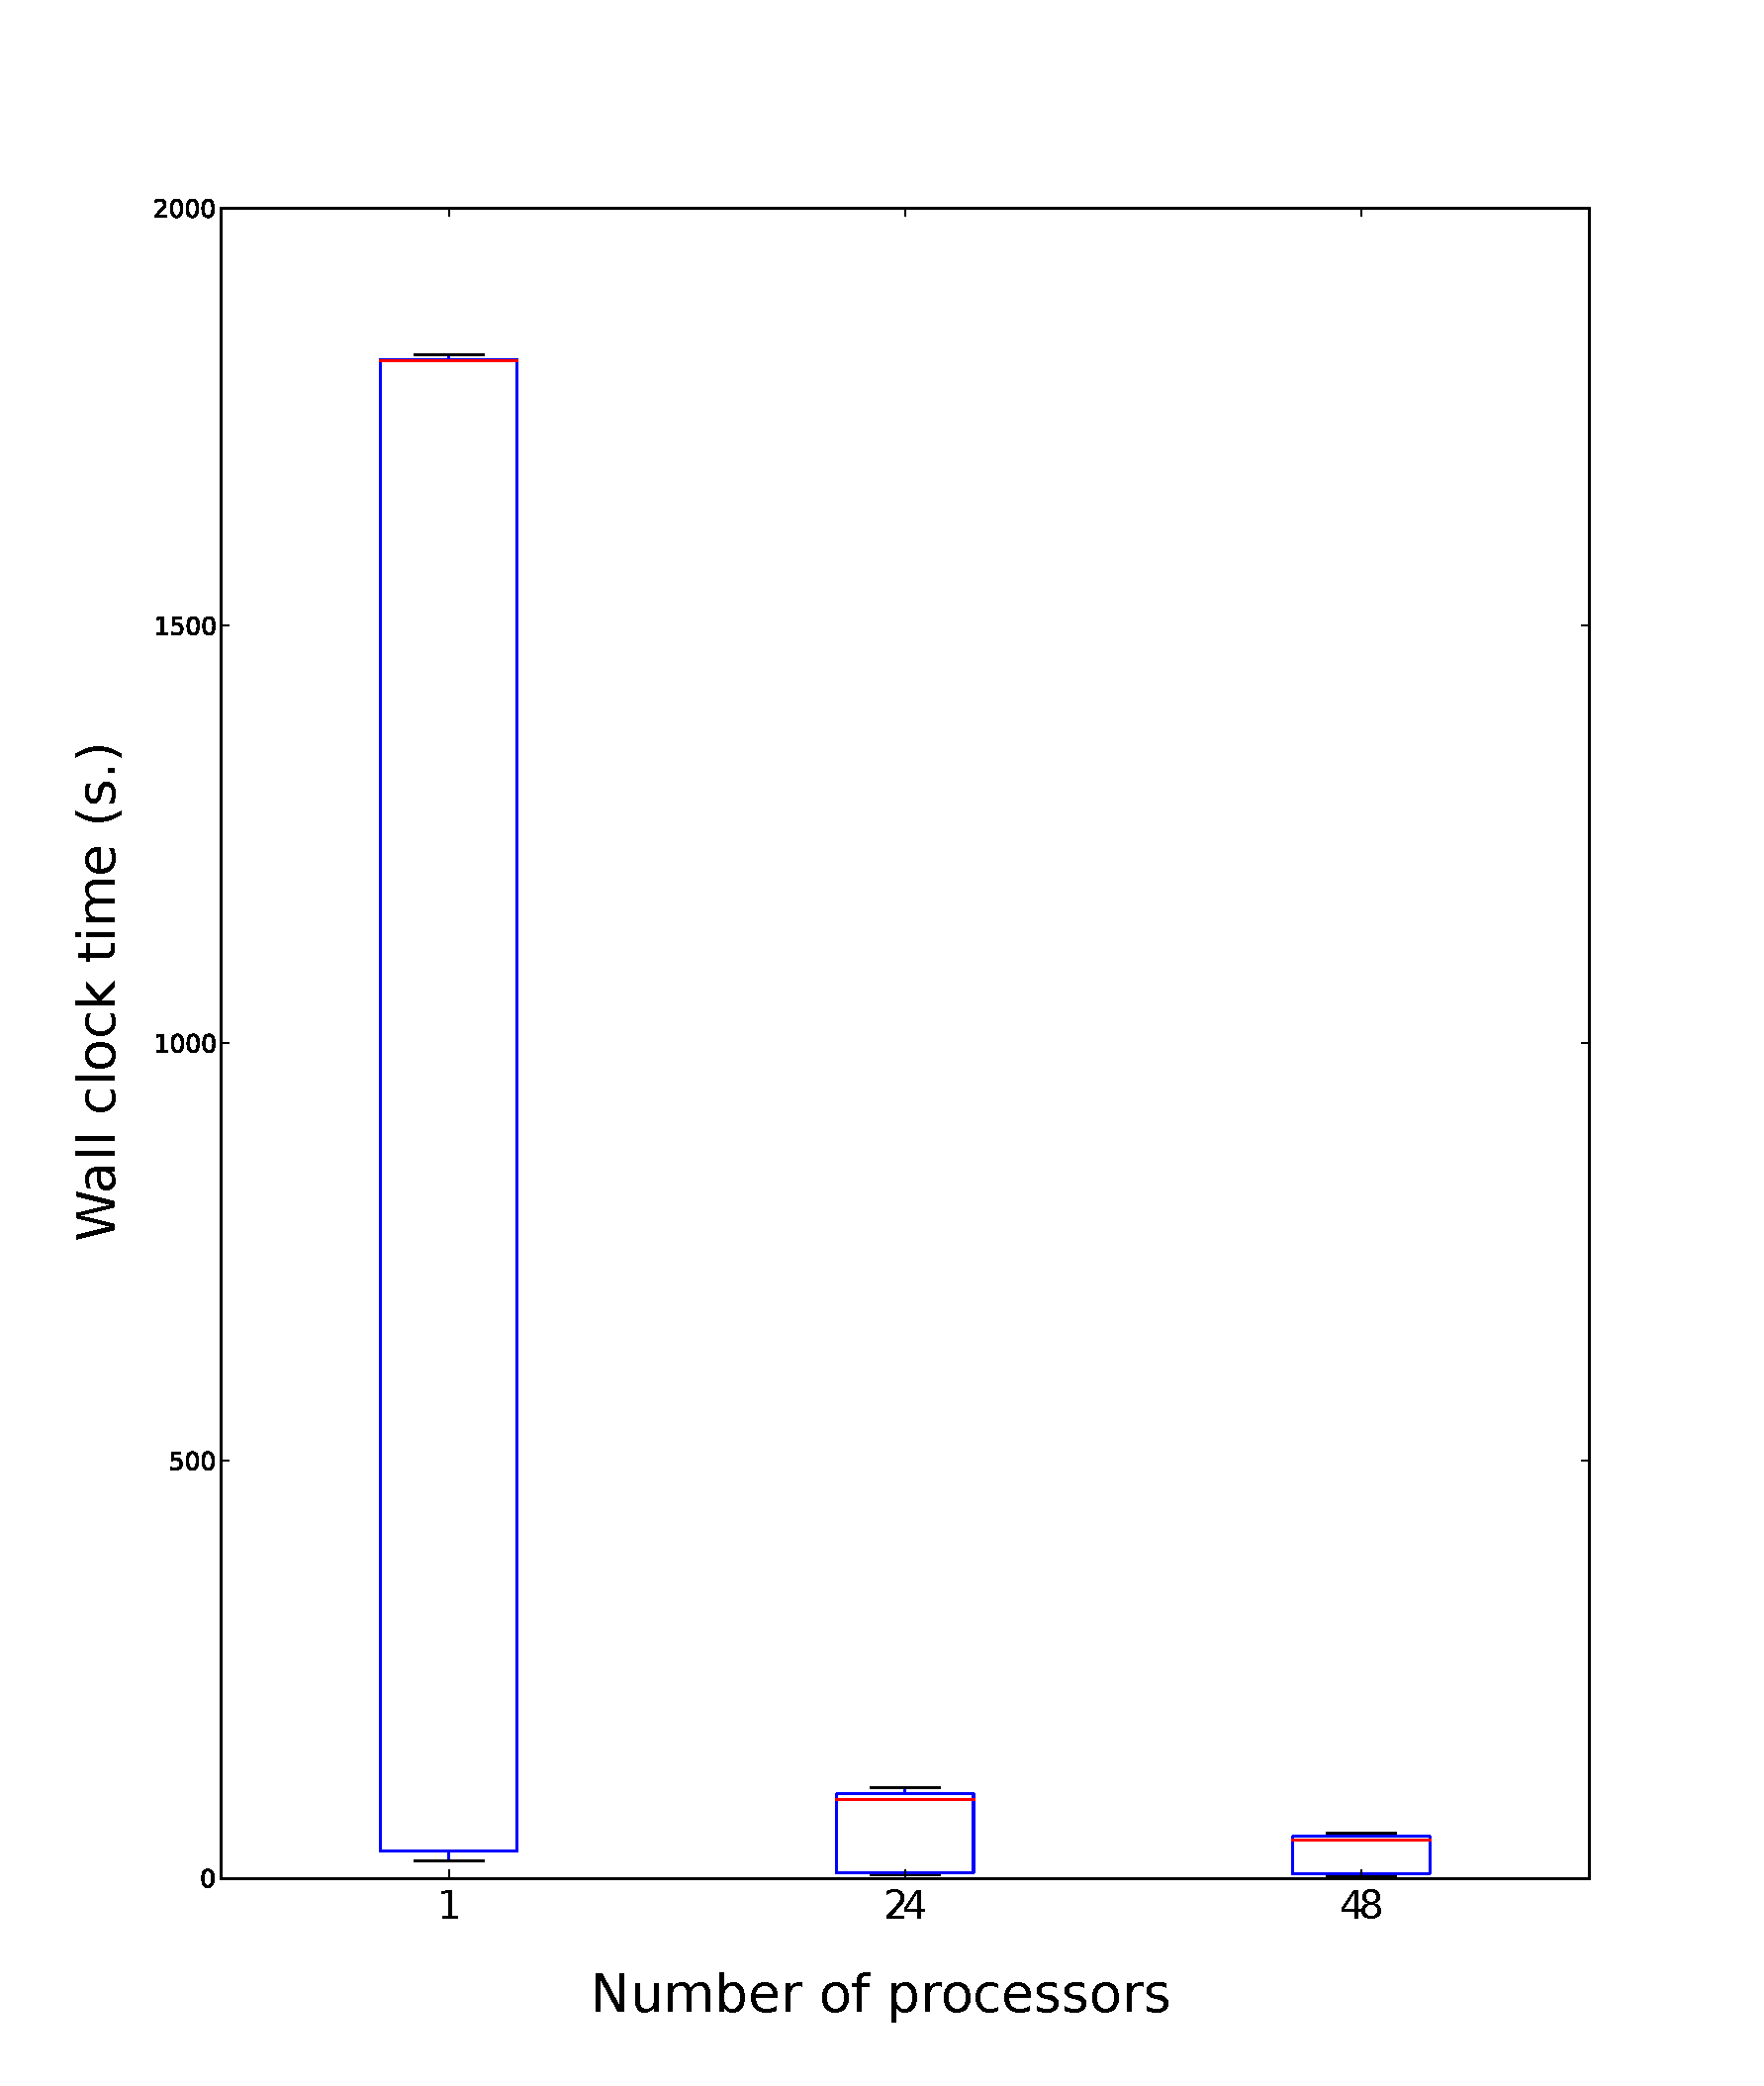
\includegraphics[width=0.2\textwidth]{images/openstacks_proc_time_dynamic.pdf}}
  \end{center}
  \caption{Absolute wallclock time distributions of 11 runs of \DAEYAHSP\ according to the number of processors, on the temporal openstacks-17 problem.}
  \label{fig:proc_static_vs_dynamic}
\end{figure}

Figure \ref{fig:proc_static_vs_dynamic} shows that the dynamic parallelization
scheme does not permits a significant speed-up comparing to the static one. The
Wilcoxon signed-rank test cannot reject the null hypothesis that the samples come
from the same distribution ($$p=0.03$$).

\paragraph{Speed-up against pop size} % (CC, JD)

\begin{figure}[htpb]
  \begin{center}
    \subfigure[full scale]{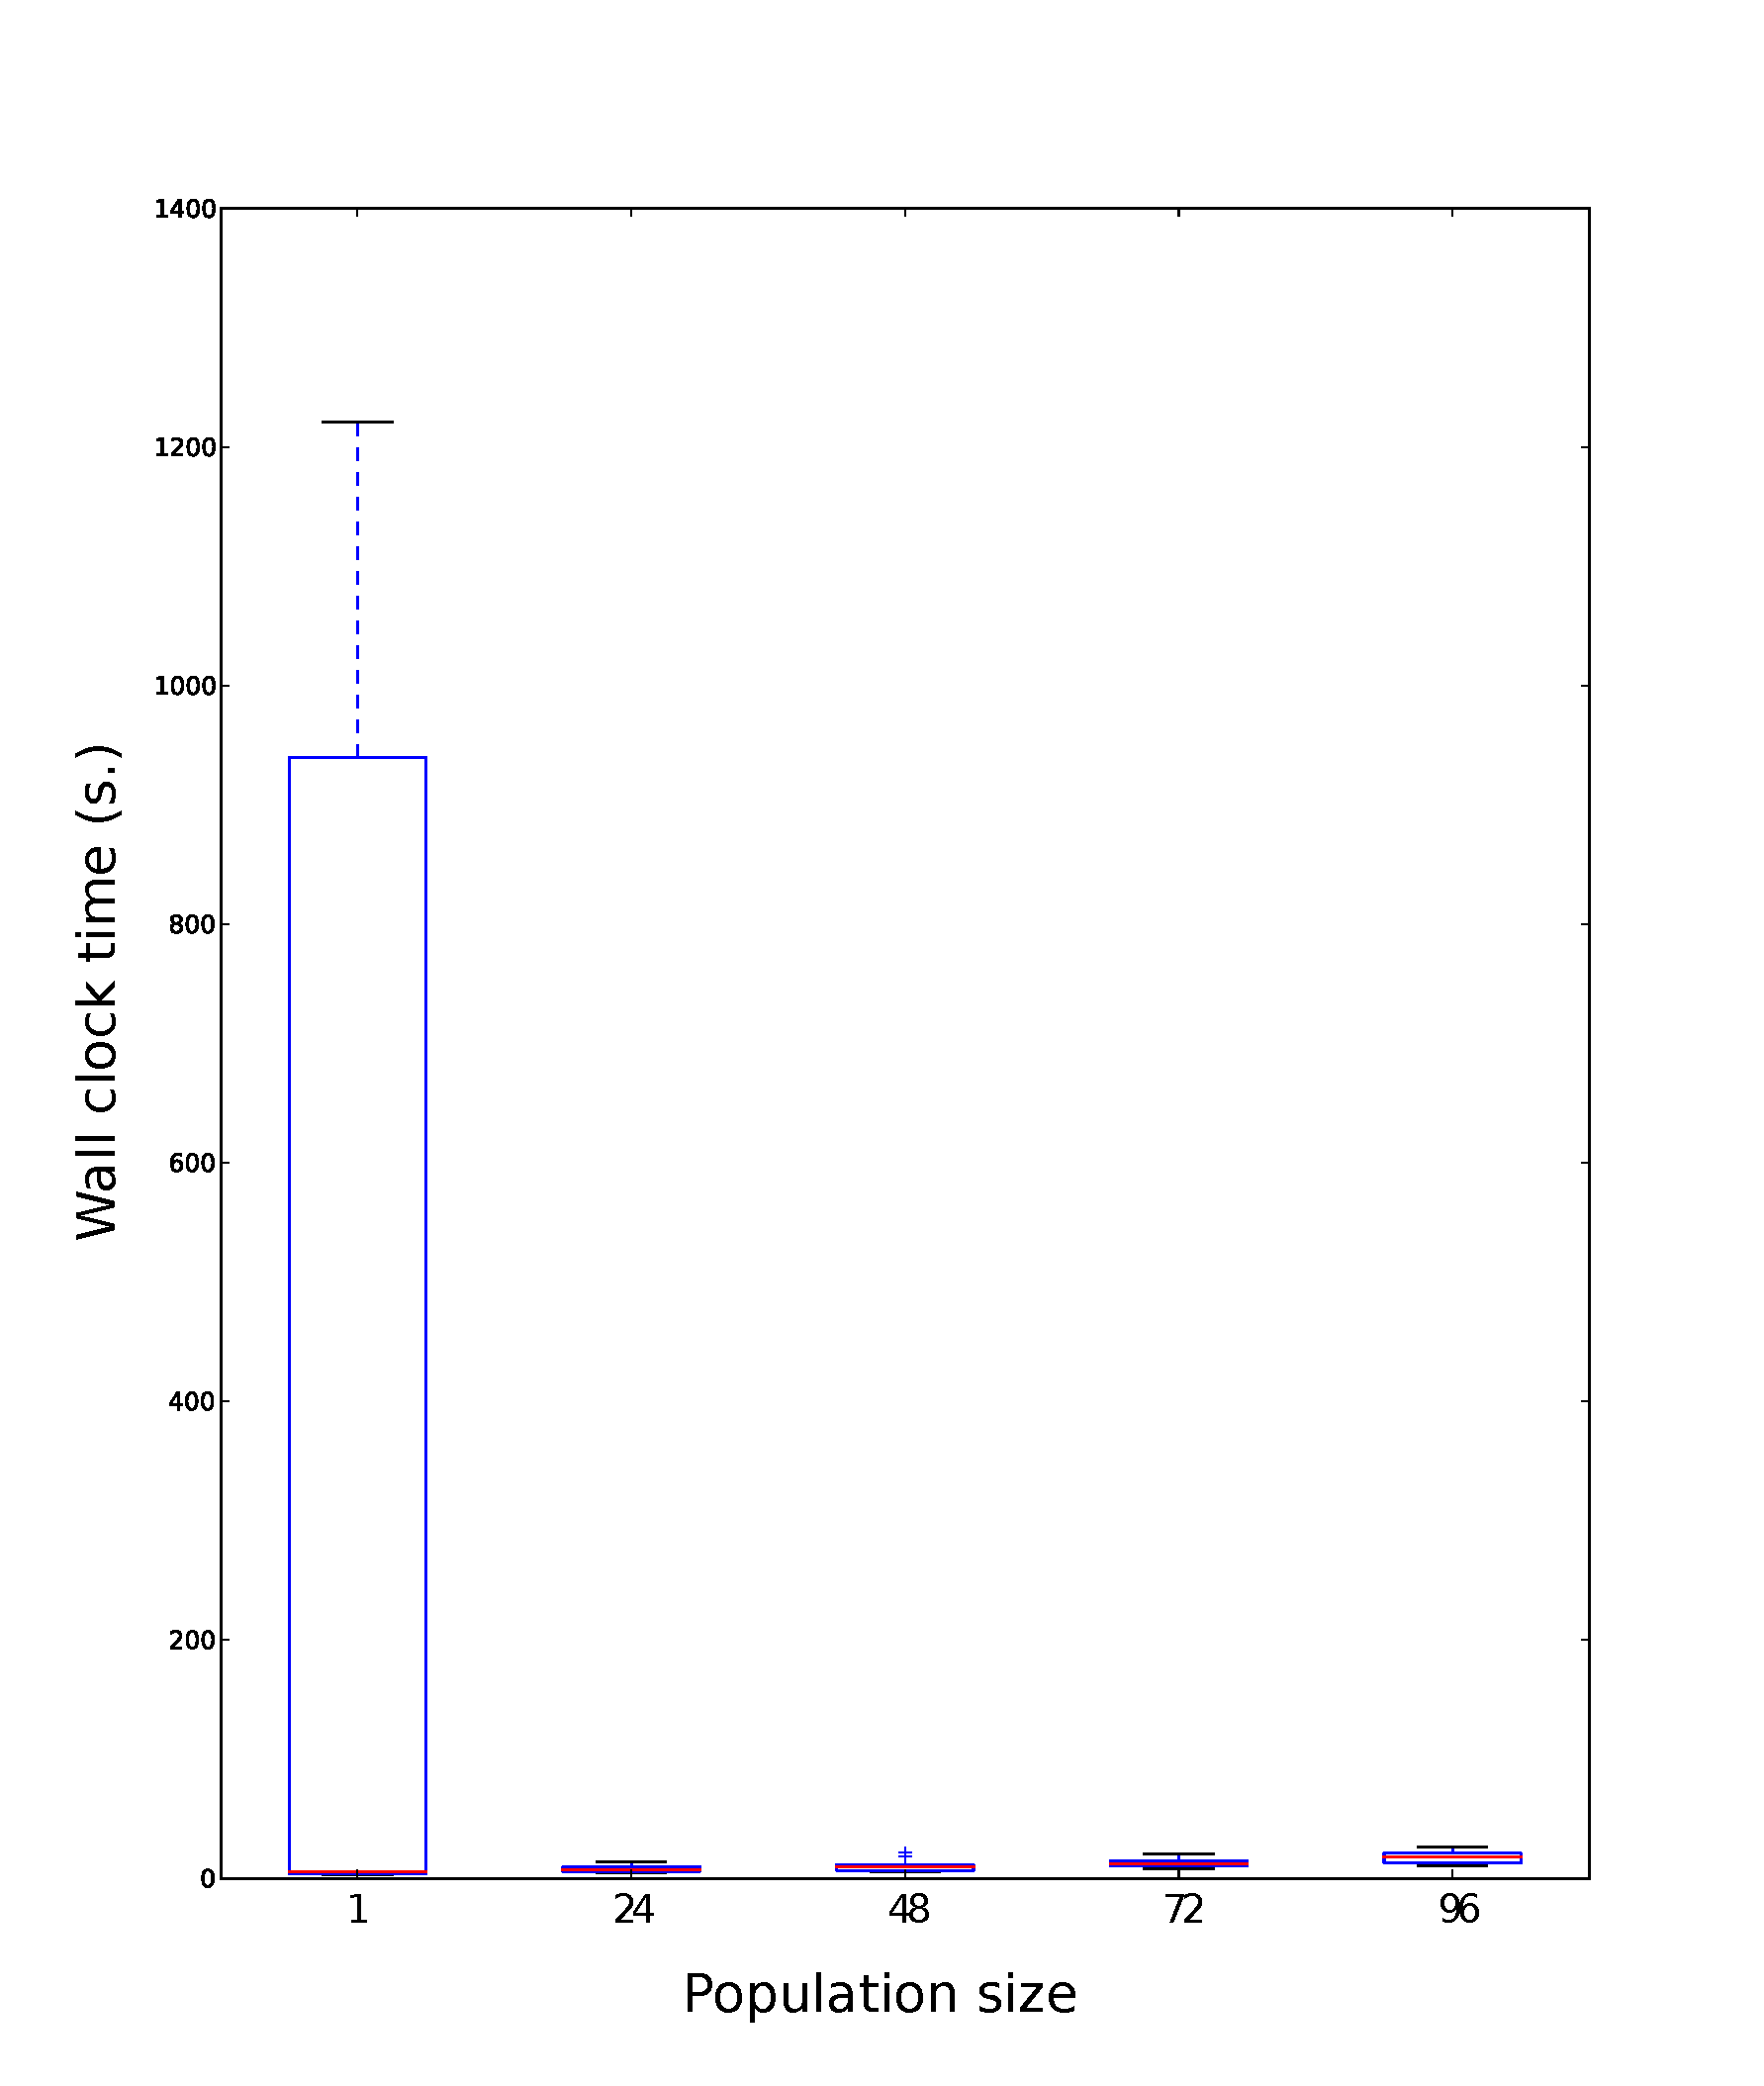
\includegraphics[width=0.2\textwidth]{images/elevators_pop_time.pdf}}
    \hfill
    \subfigure[rescaled]{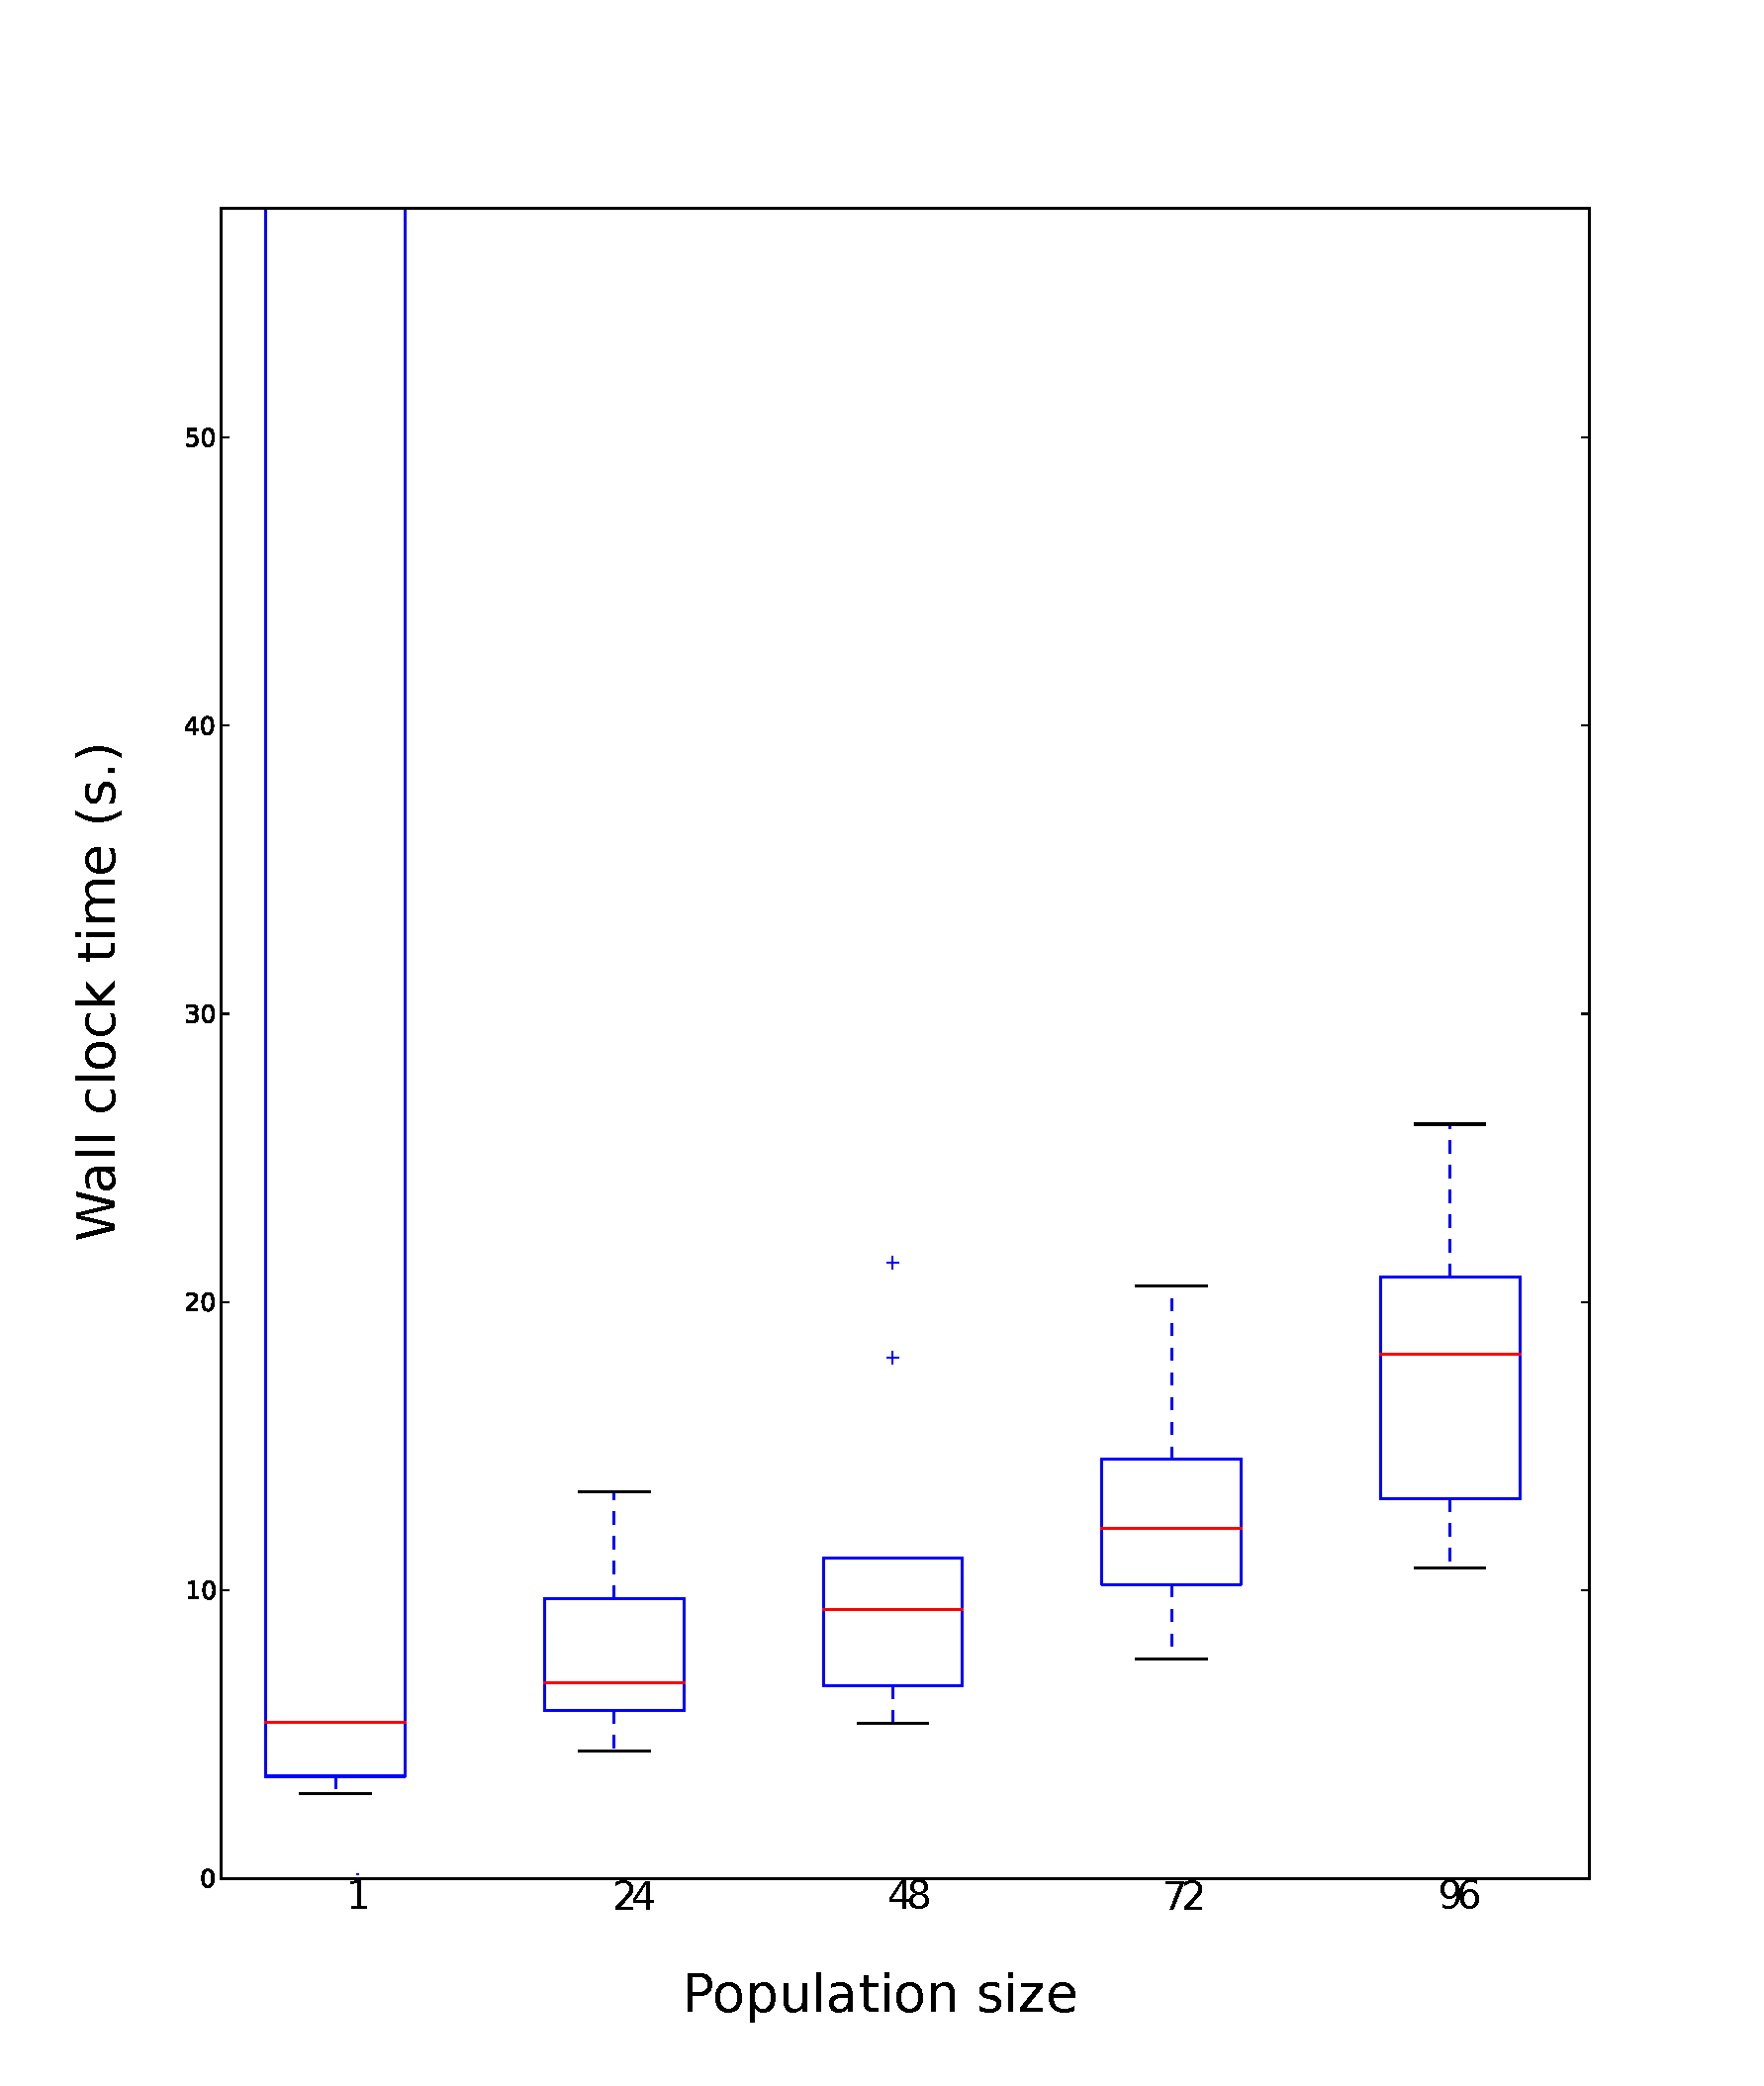
\includegraphics[width=0.2\textwidth]{images/elevators_pop_time_zoom.pdf}}
  \end{center}
  \caption{Absolute wallclock time distributions of 11 runs of \DAEYAHSP\ according to the population size, on the sequential elevators-12 problem, using 48 processors.}
  \label{fig:elevators_pop}
\end{figure}

Figure \ref{fig:elevators_pop} shows that the median computation time on a
multicore machine increase linearly with the size of the population. The 
dispersions of the distribution is due to the steady-state stopping criterion 
that may be reached after different times, with a higher probability when the
population size is small.

\section{Discussion and Conclusion}
%In order to scale up the capabilities of \DAEYAHSP, this paper investigated the parallelization of the individual evaluation.

We made a proof-of-concept of an evaluation shared-memory parallelization scheme based on the OpenMP directive-based API on a common 48-core machine.
Thanks to the abstraction level provided by the EO framework, this scheme is immediately available for any evolutionary algorithm as far as the individual local context is protected.

The implementation scheme presented here is very simple, but works extremely well.
A further development will consist in parallelizing other steps of the evolutionary loop in particular the offspring generation which is also inherently parallel.
On our 48-core Dell Machine a roughly $\times40$ was obtained on the two benchmarks tested.

The queue mapping management of threads onto cores did not provide a significant improvement. Our hypothesis was that the goal sequences shows a diversity in length and thus should have shown very diverse times of evaluation computations. But we observed that the algorithm converges rapidly to a same length for all individuals.

% Impact on the EA design

A further research axis deals with the impact on solution quality and in particular how to escape from premature convergence.







%ACKNOWLEDGMENTS are optional
%\section{Acknowledgments}

%
% The following two commands are all you need in the
% initial runs of your .tex file to
% produce the bibliography for the citations in your paper.
\bibliographystyle{abbrv}
\bibliography{dae_mt}  % sigproc.bib is the name of the Bibliography in this case
% You must have a proper ".bib" file
%  and remember to run:
% latex bibtex latex latex
% to resolve all references
%
% ACM needs 'a single self-contained file'!
%
%Generated by bibtex from your ~.bib file.  Run latex,
%then bibtex, then latex twice (to resolve references)
%to create the ~.bbl file.  Insert that ~.bbl file into
%the .tex source file and comment out
%the command \texttt{{\char'134}thebibliography}.
\end{document}

\DAE\ has been implemented within the Evolving Objects framework (\url{http://eodev.sourceforge.net/}), an Open Source, STL-based, C++ Evolutionary Computation library. 
The fixed {\em evolution engine} is a (100+700)-ES: 100 individuals generate 700 offsprings without selection. The survival selection is performed among those 800 individuals using a {\em deterministic tournament} of size 5. For all runs, the {\bf stopping criterion} is the following: After at least 10 generations, evolution is stopped if no improvement of the best fitness in the population is made during 50 generations, with a maximum of 1000 generations. Furthermore, all runs were allowed a maximum CPU time of 30mn (running on 3.4 GHz cores).


Multicore machines are becoming a standard way to speep up the system performance.

This paper describes a multi-threaded release of \DAEYAHSP.

This paper describes a parallel shared-memory release of the \DAEYAHSP\ planning system.
using the OpenMP directive-based API.

to obtain high levels of performance special care has been given to get reentrant procedures.
isolate context variables 

% concurrent programming

OpenMP primarily consists of a set of compiler directives (pragmas) that are inserted into a Fortran, C or C++ program to convey information to an OpenMP compiler.


\cite{paradiseo:JHeuristics2004}
\cite{paradiseo:ParallelComputing2004}
\cite{alba:IEEE2002}
\cite{alba:COR2008}
\cite{alba:IPL2002}
\cite{dae:icaps2010}
\cite{dae:evocop2006}
\cite{dae:gecco2010}

In order to scale up the capabilities of \DAEYAHSP, this paper investigated the parallelization of the individual evaluation.
